\documentclass[a4paper,10pt]{article}
\usepackage[margin=1in]{geometry}
\usepackage{graphicx}
\usepackage{amsmath}
\usepackage{listings}
\usepackage{xcolor}
\usepackage{pythonhighlight}
\usepackage{caption}  % Added for figure captions
\usepackage{setspace} % For line spacing
\usepackage{array} % For table formatting
\setstretch{1} % Reduce line spacing to 1

% Define colors for code
\definecolor{bg}{rgb}{0.95,0.95,0.95}
\definecolor{comment}{rgb}{0.5,0.5,0.5}
\definecolor{keyword}{rgb}{0.25,0.5,0.75}
\definecolor{string}{rgb}{0.5,0.25,0.25}

% Set up code listings
\lstset{
    backgroundcolor=\color{bg},
    basicstyle=\ttfamily,
    commentstyle=\color{comment},
    keywordstyle=\color{keyword},
    stringstyle=\color{string},
    breaklines=true,
    frame=single,
    tabsize=4,
    captionpos=b
}

\begin{document}
\vspace{-2cm}
\title{\LARGE \textbf{TRINITY COLLEGE DUBLIN} \\ % Reduced space between title and next line
\large School of Computer Science and Statistics \\
\small \textbf{CS7CS4/CSU44061 Machine Learning}}
\author{Abhishek Zade}
\date{} % Optionally remove date if not needed
\maketitle
\vspace{-1cm} % Adjust this value to reduce space between the author and title

\noindent
\textbf{StudentId:} 24332461 \\
\textbf{Dataset-1 id:} \# id:12-24-12-1 \\
\textbf{Dataset-2 id:} \# id:12-12-12-1 \\
\textbf{Week 4 Assignment} \\

% Horizontal line
\noindent\rule{\textwidth}{0.4pt} % This creates a horizontal line across the width of the page

\section*{Model Solution}

\subsection*{(i)}
\begin{enumerate}
    \item[(a)]   
The graph in figure 1 displays the average F1 score for a logistic regression model with varying values of $C$ (regularisation strength) and polynomial degrees 1 to 7. Stable performance is shown by degrees 2 and 3, which consistently obtain the greatest F1 score of about 0.80 across all values of $C$. Higher polynomial degrees (6 and 7) indicate instability or overfitting since they exhibit slightly lower F1 scores and more variability. A polynomial degree of two or three with a $C$ value of one or higher is the ideal combination for simplicity and performance.    \begin{center}
        \centering
        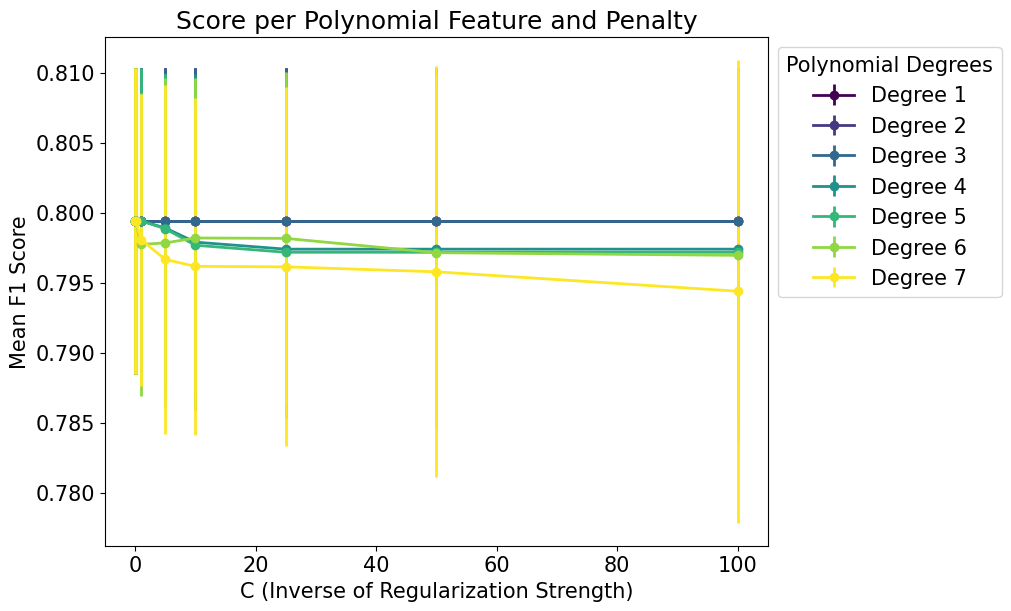
\includegraphics[width=0.75\linewidth]{a.1.png}
        \captionof{figure}{Impact of C Values and Polynomial Complexity on Logistic Regression Performance}
        \label{}
    \end{center}
\item[(b)]   
The graph shows in the figure 2 represents k-Nearest Neighbours (kNN) model's average F1 score for a range of $K$ (number of neighbours) values. After a considerable increase from $K = 1$ to roughly $K = 20$, the F1 score stabilises at 0.80. The best performance occurs between $K = 10$ and $K = 20$, where the error bars are comparatively tiny and the F1 score is high and steady. The F1 score stays constant as $K$ rises, however there are minor increases in variability, suggesting possible underfitting. For the optimum performance, I suggest a $K$ value of 1 or higher, between 10 and 20.    
       \begin{center}
        \centering
        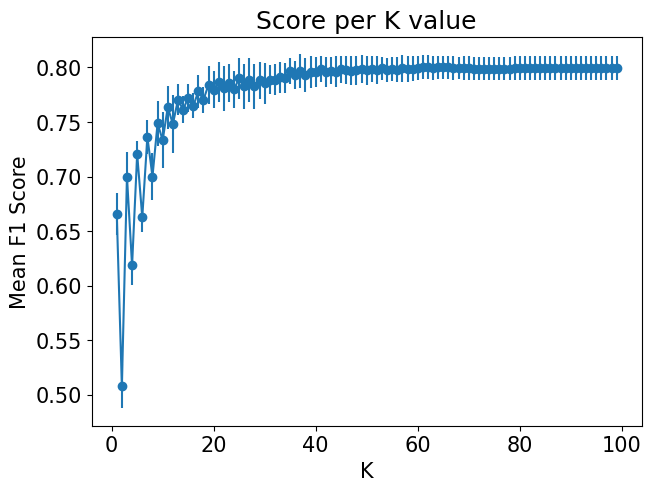
\includegraphics[width=0.75\linewidth]{a.2.png}
        \captionof{figure}{Impact of K Value on k-Nearest Neighbors Model Performance}
        \label{}
    \end{center} 

\item[(c)] \textbf{Confusion Matrix and Classification Report} \\
\begin{table}[ht]
    \centering
    \caption{Confusion Matrices for All Models}
    \begin{tabular}{l|cc|cc|cc|cc}
        \hline
        & \multicolumn{2}{c|}{Logistic Regression} & \multicolumn{2}{c|}{kNN} & \multicolumn{2}{c|}{Random Model} & \multicolumn{2}{c}{Most Frequent} \\
        \hline
        & Pred -1 & Pred 1 & Pred -1 & Pred 1 & Pred -1 & Pred 1 & Pred -1 & Pred 1 \\
        \hline
        Actual -1 & 0 & 483 & 77 & 406 & 240 & 243 & 0 & 483 \\
        Actual 1  & 0 & 963 & 59 & 904 & 484 & 479 & 0 & 963 \\
        \hline
    \end{tabular}
    \label{tab:confusion_matrices}
\end{table}
\begin{table}[ht]
    \centering
    \caption{Classification Reports for All Models}
    \begin{tabular}{l|c|c|c|c}
        \hline
        Metric & Logistic Regression & kNN & Random Model & Most Frequent \\
        \hline
        Precision (-1) & 0.00 & 0.57 & 0.33 & 0.00 \\
        Recall (-1)    & 0.00 & 0.16 & 0.50 & 0.00 \\
        F1-score (-1)  & 0.00 & 0.25 & 0.40 & 0.00 \\
        Precision (1)  & 0.67 & 0.69 & 0.66 & 0.67 \\
        Recall (1)     & 1.00 & 0.94 & 0.50 & 1.00 \\
        F1-score (1)   & 0.80 & 0.80 & 0.57 & 0.80 \\
        Accuracy       & 0.67 & 0.68 & 0.50 & 0.67 \\
        Macro avg Precision & 0.33 & 0.63 & 0.50 & 0.33 \\
        Macro avg Recall    & 0.50 & 0.55 & 0.50 & 0.50 \\
        Macro avg F1-score  & 0.40 & 0.52 & 0.48 & 0.40 \\
        Weighted avg Precision & 0.44 & 0.65 & 0.55 & 0.44 \\
        Weighted avg Recall    & 0.67 & 0.68 & 0.50 & 0.67 \\
        Weighted avg F1-score  & 0.53 & 0.61 & 0.51 & 0.53 \\
        \hline
    \end{tabular}
    \label{tab:classification_reports}
\end{table} \\

\newpage
\item[(d)] \textbf{Performance Analysis of Classifiers Using ROC Curves}
 \begin{center}
        \centering
        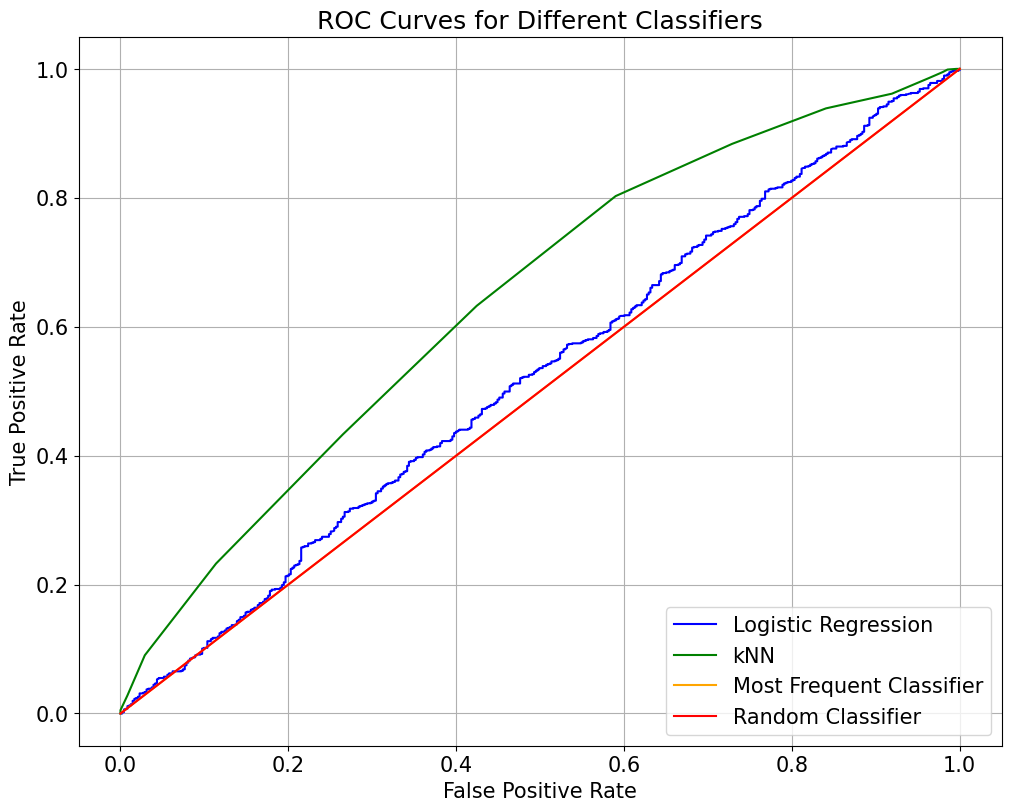
\includegraphics[width=0.75\linewidth]{a.3.png}
        \captionof{figure}{ROC Curves for Logistic Regression, kNN, Most Frequent, and Random Classifiers}
        \label{}
    \end{center}
    According to Tables 1 and 2, the Logistic Regression model exhibited an accuracy of 67\% and an F1-score of 0.80 for class $1$, but no predictive power for class $-1$. The accuracy of the kNN Classifier was marginally higher at 68\%, with an F1-score of 0.25 for class $-1$ and 0.80 for class $1$. The Random Model achieved 50\% accuracy and performed moderately, with F1-scores of 0.40 for class $-1$ and 0.57 for class $1$. The accuracy of the Most Frequent Classifier was 67\%, since it only predicted class $1$. The better performance of the kNN and logistic regression classifiers was confirmed by the lower F1 scores and larger variability of both baseline models.

\item[(e)]
As seen in Figure 1, the Logistic Regression model with polynomial degree 3 and $C = 5$ offered the best results by striking a balance between complexity and variance. Figure 2 illustrates how the kNN Classifier with $K = 22$ produced consistent results without overfitting or underfitting. The accuracy of the kNN Classifier was 68\%, whereas that of the Logistic Regression was 67\%. With non-zero F1-scores for both classes (0.25 for $-1$ and 0.80 for $1$), the kNN model demonstrated a superior balance. On the other hand, class $-1$ was difficult for the Most Frequent and Logistic Regression models to forecast. The accuracy of the Random Model was 50\%, which was a moderate performance. Because of its greater AUC, accuracy, and class balance, kNN is suggested for this assignment based on the ROC curves, which show its significant discriminative capacity. 
\end{enumerate}
\subsection*{(ii)}
\begin{enumerate}
    \item[(a)] 
    The mean Logistic Regression F1 score for various polynomial degrees and regularisation values $C$ is displayed in Figure 4. Finding degree 4 and $C = 10$ as the ideal values is made easier by the error bars, which show variability between folds. Across all values of $C$, polynomial degrees between 2 and 7 in Figure 4 consistently obtain excellent F1 scores near 0.98, demonstrating dependable performance. Particularly for low $C$, Degree 1 performs poorly, with an F1 score of around 0.90 and more variability. The results of the kNN cross validation are shown in Figure 5, where the most stable value is $K = 30$. Overall, polynomial degrees 2 through 7 are the best option since they show the least fluctuation and performance that is consistently high.performance.    
\begin{center}
        \centering
        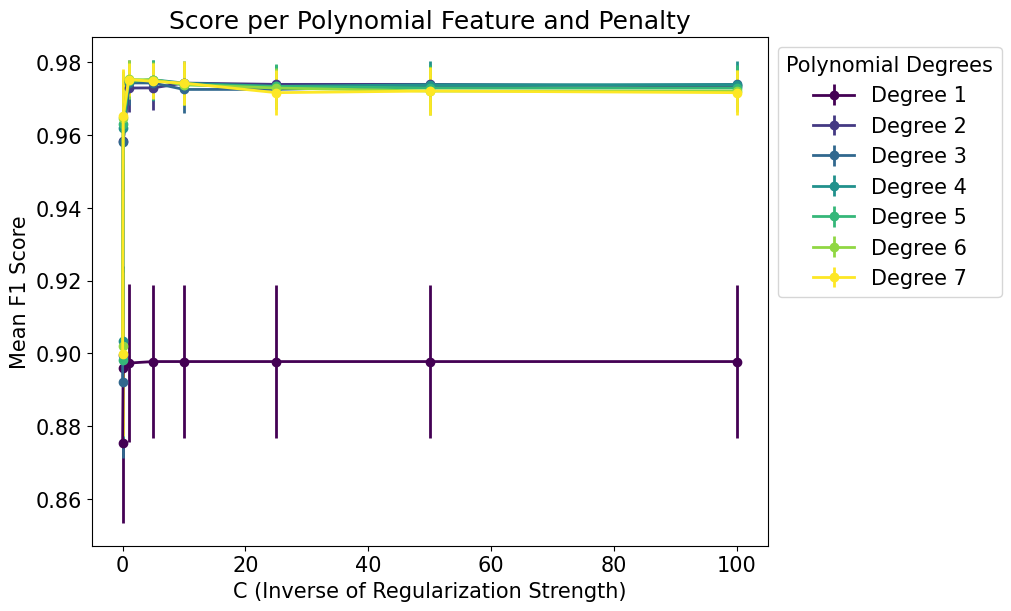
\includegraphics[width=0.75\linewidth]{b.1.png}
        \captionof{figure}{Impact of C Values and Polynomial Complexity on Logistic Regression Performance}
        \label{}
    \end{center}
\item[(b)]   
The average F1 score for a k-Nearest Neighbours (kNN) classifier with different $K$ values is displayed in the figure 5 graph. After rising initially, the F1 score peaks between $K = 15$ and $25$, when it is nearly $0.98$. Next, while $K$ keeps rising, the F1 score starts to marginally decline, suggesting that over-smoothing may be causing the model to perform worse. Additionally, with smaller values of $K$, the variance is bigger, suggesting less stability.    
       \begin{center}
        \centering
        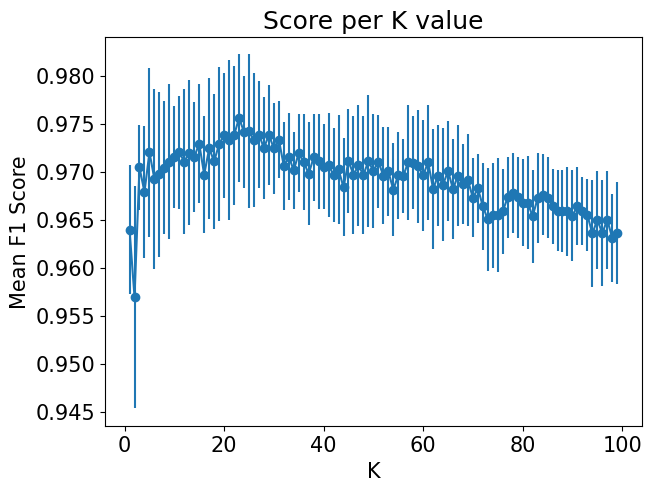
\includegraphics[width=0.75\linewidth]{b.2.png}
        \captionof{figure}{Impact of K Value on k-Nearest Neighbors Model Performance}
        \label{}
    \end{center} 

\item[(c)] \textbf{Confusion Matrix and Classification Report} \\
\begin{table}[ht]
    \centering
    \caption{Confusion Matrices for All Models}
    \begin{tabular}{l|cc|cc|cc|cc}
        \hline
        & \multicolumn{2}{c|}{Logistic Regression} & \multicolumn{2}{c|}{kNN} & \multicolumn{2}{c|}{Random Model} & \multicolumn{2}{c}{Most Frequent} \\
        \hline
        & Pred -1 & Pred 1 & Pred -1 & Pred 1 & Pred -1 & Pred 1 & Pred -1 & Pred 1 \\
        \hline
        Actual -1 & 530 & 28 & 535 & 23 & 265 & 293 & 0 & 558 \\
        Actual 1  & 24 & 1090 & 34 & 1080 & 579 & 535 & 0 & 1114 \\
        \hline
    \end{tabular}
    \label{tab:confusion_matrices}
\end{table}

\begin{table}[ht]
    \centering
    \caption{Classification Reports for All Models}
    \begin{tabular}{l|c|c|c|c}
        \hline
        Metric & Logistic Regression & kNN & Random Model & Most Frequent \\
        \hline
        Precision (-1) & 0.96 & 0.94 & 0.31 & 0.00 \\
        Recall (-1)    & 0.95 & 0.96 & 0.47 & 0.00 \\
        F1-score (-1)  & 0.95 & 0.95 & 0.38 & 0.00 \\
        Precision (1)  & 0.97 & 0.98 & 0.65 & 0.67 \\
        Recall (1)     & 0.98 & 0.97 & 0.48 & 1.00 \\
        F1-score (1)   & 0.98 & 0.97 & 0.55 & 0.80 \\
        \hline
        Accuracy       & 0.97 & 0.97 & 0.48 & 0.67 \\
        Macro avg Precision & 0.97 & 0.96 & 0.48 & 0.33 \\
        Macro avg Recall    & 0.96 & 0.96 & 0.48 & 0.50 \\
        Macro avg F1-score  & 0.96 & 0.96 & 0.46 & 0.40 \\
        Weighted avg Precision & 0.97 & 0.97 & 0.54 & 0.44 \\
        Weighted avg Recall    & 0.97 & 0.97 & 0.48 & 0.67 \\
        Weighted avg F1-score  & 0.97 & 0.97 & 0.49 & 0.53 \\
        \hline
    \end{tabular}
    \label{tab:classification_reports}
\end{table}
Both the Logistic Regression and kNN classifiers had strong precision, recall, and F1-scores for both classes (-1 and 1), and both achieved an accuracy of 97\%. With an accuracy of 48\%, the Random Model performed noticeably worse and produced uneven outcomes across classes. Although it only predicted the majority class, the Most Frequent Classifier had a 67\% accuracy rate, meaning it performed poorly for class $-1$. Random and Most Frequent classifiers perform much worse than Logistic Regression and kNN, which are the best-performing models overall.

\item[(d)] \textbf{Performance Analysis of Classifiers Using ROC Curves}
 \begin{center}
        \centering
        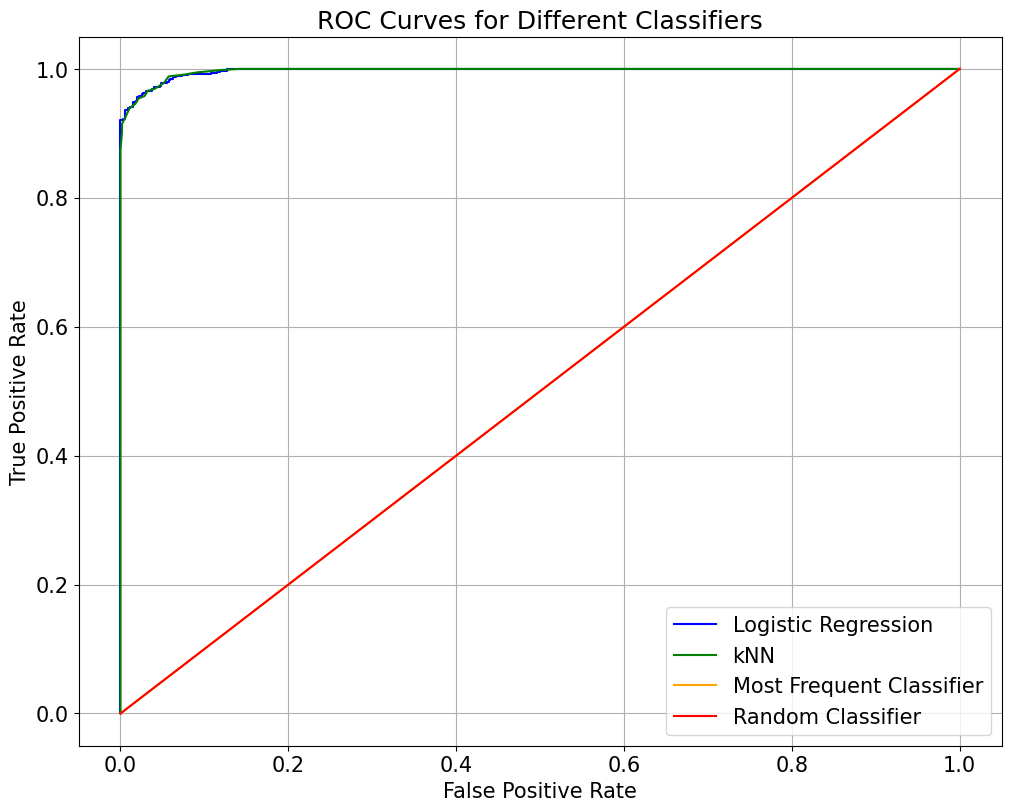
\includegraphics[width=0.75\linewidth]{b.3.png}
        \captionof{figure}{ROC Curves for Logistic Regression, kNN, Most Frequent, and Random Classifiers}
        \label{}
    \end{center} 
    The second dataset's ROC curves, which compare the Random Classifier, Most Frequent Classifier, kNN, and Logistic Regression, are shown in Figure 6. With the highest AUC of 0.97, the kNN Classifier demonstrated great discriminative ability, whereas Logistic Regression performed competitively with an AUC of 0.94. The ROC curves for both kNN and logistic regression approach the upper-left corner of Figure 6, indicating low false positive rates and high true positive rates. The Most Frequent and Random Classifiers, on the other hand, display ROC curves along the diagonal, indicating a lack of discriminative power and random guessing. In terms of class distinction, kNN and Logistic Regression perform noticeably better than the baseline classifiers.
\item[(e)]
For the second dataset, I selected the Logistic Regression model with polynomial degree 4 and $C = 10$ (Figure 4), which provided strong cross-validation performance and struck the perfect balance between generalisability and complexity. I saw that the kNN Classifier with $K = 30$ in Figure 5 had the highest mean F1 score and the lowest variance, indicating good model behaviour. Both models achieved 97\% accuracy with balanced precision, recall, and F1-scores for classes $-1$ and $1$, indicating their strong ability to distinguish between the two classes. The Most Frequent Classifier has an F1-score of 0.00 since it could not predict class $-1$, even with an accuracy of 67\%. With an accuracy of 48\% and inconsistent forecasts across courses, the Random Model fared even worse. Both kNN and Logistic Regression outperformed the baseline models, which were very equivalent to random guessing, as seen by the ROC curves in Figure 6. Because of its somewhat better stability, less variance, and consistent results across classes, I recommend the kNN Classifier as the best model for this dataset.
\end{enumerate}
\begin{lstlisting}[language=Python, caption={}]
# for dataId : # id:12-24-12-1
import numpy as np
import pandas as pd
import matplotlib.pyplot as plt
from sklearn.preprocessing import PolynomialFeatures
from sklearn.linear_model import LogisticRegression
from sklearn.model_selection import KFold
from sklearn.metrics import f1_score
from sklearn.neighbors import KNeighborsClassifier
from sklearn.metrics import confusion_matrix
from sklearn.metrics import classification_report
from sklearn.dummy import DummyClassifier
from sklearn.metrics import roc_curve
df = pd.read_csv("./data/week4_1.csv")
df.columns = ['X1', 'X2', 'y']
df.head()
X1 = df['X1']
X2 = df['X2']
X = np.column_stack((X1, X2))
y = df['y']
point = np.column_stack((X1, X2, y))
plt.scatter(X1[y == 1], X2[y == 1], marker='+', c='blue', label="Positive", alpha=0.8, edgecolors='w')
plt.scatter(X1[y == -1], X2[y == -1], marker='o', c='orange', label='Negative', alpha=0.8)
plt.xlabel('X1')
plt.ylabel('X2')
plt.title('Data')
plt.legend(loc='upper right')
plt.show()
def logisticRegressionKFold(x, y, poly_degrees, C_range, k_fold_value):
    plt.figure(figsize=(10, 6))
    colors = plt.cm.viridis(np.linspace(0, 1, len(poly_degrees)))
    for idx, degree in enumerate(poly_degrees):
        mean_error = []
        std_error = []
        x_poly = PolynomialFeatures(degree).fit_transform(x)
        for C in C_range:   
            LRModel = LogisticRegression(penalty='l2', C=C, solver='lbfgs', max_iter=1000)
            k_fold = KFold(n_splits=k_fold_value, shuffle=True, random_state=42)
            f1_scores = []
            for train_index, test_index in k_fold.split(x_poly):
                LRModel.fit(x_poly[train_index], y[train_index])
                y_pred = LRModel.predict(x_poly[test_index])
                f1 = f1_score(y[test_index], y_pred)
                f1_scores.append(f1)        
            mean_error.append(np.mean(f1_scores))
            std_error.append(np.std(f1_scores))
        plt.errorbar(C_range, mean_error, yerr=std_error, label=f'Degree {degree}',
                     color=colors[idx], fmt='-o', linewidth=2, markersize=6)
    plt.xlabel('C (Inverse of Regularization Strength)')
    plt.ylabel('Mean F1 Score')
    plt.title('Score per Polynomial Feature and Penalty')
    plt.legend(title='Polynomial Degrees', bbox_to_anchor=(1, 1))
    plt.show()
# This values I am taking from last assignments according what i have understand    
poly_degree = [1, 2, 3, 4, 5, 6, 7]
C_range = [0.01, 0.1, 1, 5, 10, 25, 50, 100]
k_fold_value = 5
logisticRegressionKFold(X, y, poly_degree, C_range, k_fold_value)
def knearestNeighborKFold(k_range, x, y, k_fold_value):
    mean_error = []
    std_error = []   
    for k in k_range:
        model = KNeighborsClassifier(n_neighbors=k)
        k_fold = KFold(n_splits=k_fold_value, shuffle=True, random_state=42)
        f1_scores = []
        for train_index, test_index in k_fold.split(x):        
            model.fit(x[train_index], y[train_index])
            y_pred = model.predict(x[test_index])
            f1 = f1_score(y[test_index], y_pred)
            f1_scores.append(f1)
        mean_error.append(np.mean(f1_scores))
        std_error.append(np.std(f1_scores))
    plt.errorbar(k_range, mean_error, yerr=std_error, fmt='-o')
    plt.xlabel('K')
    plt.ylabel('Mean F1 Score')
    plt.title('Score per K value')
    plt.show()
k_range = np.array(range(1, 100))
k_fold_value = 5
knearestNeighborKFold(k_range, X, y, k_fold_value)
best_degree = 3
best_C = 5
poly = PolynomialFeatures(best_degree)
x_poly = poly.fit_transform(X)
logistic_model = LogisticRegression(penalty='l2', C=best_C, max_iter=1000)
logistic_model.fit(x_poly, y)
y_pred_logistic = logistic_model.predict(x_poly)
conf_matrix_logistic = confusion_matrix(y, y_pred_logistic)
class_matrix_logistic = classification_report(y, y_pred_logistic)
print("Confusion Matrix for Logistic Regression:")
print(conf_matrix_logistic)
print("Classification Report for Logistic Regression:")
print(class_matrix_logistic)
best_k = 22
knn_model = KNeighborsClassifier(n_neighbors=best_k)
knn_model.fit(X, y)
y_pred_knn = knn_model.predict(X)
conf_matrix_knn = confusion_matrix(y, y_pred_knn)
class_matrix_knn = classification_report(y, y_pred_knn)
print("\nConfusion Matrix for kNN Classifier:")
print(conf_matrix_knn)
print("Classification Report for kNN Classifier:")
print(class_matrix_knn)
random_model = DummyClassifier(strategy="uniform", random_state=42).fit(X, y)
random_predictions = random_model.predict(X)
print("Confusion Matrix for Random Model:\n")
print(confusion_matrix(y, random_predictions))
print("\nClassification Report for Random Model:\n")
print(classification_report(y, random_predictions))
most_frequent_model = DummyClassifier(strategy="most_frequent").fit(X, y)
most_frequent_predictions = most_frequent_model.predict(X)
print("\nConfusion Matrix for Most Frequent Model:\n")
print(confusion_matrix(y, most_frequent_predictions))
print("\nClassification Report for Most Frequent Model:\n")
print(classification_report(y, most_frequent_predictions))
LR_decision_function = logistic_model.decision_function(x_poly)
fpr, tpr, _ = roc_curve(y, LR_decision_function)
knn_probability = knn_model.predict_proba(X)
most_frequent_probability = most_frequent_model.predict_proba(X)
random_probability = random_model.predict_proba(X)
knn_fpr, knn_tpr, _ = roc_curve(y, knn_probability[:, 1])
most_freq_fpr, most_freq_tpr, _ = roc_curve(y, most_frequent_probability[:, 1])
rand_fpr, rand_tpr, _ = roc_curve(y, random_probability[:, 1])
plt.figure(figsize=(10, 8))
plt.plot(fpr, tpr, label='Logistic Regression', color='blue')
plt.plot(knn_fpr, knn_tpr, label='kNN', color='green')
plt.plot(most_freq_fpr, most_freq_tpr, label='Most Frequent Classifier', color='orange')
plt.plot(rand_fpr, rand_tpr, label='Random Classifier', color='red')
plt.xlabel('False Positive Rate')
plt.ylabel('True Positive Rate')
plt.title('ROC Curves for Different Classifiers')
plt.legend(loc='lower right')
plt.grid()
plt.show()

# for dataId : # id:12-12-12-1
df = pd.read_csv("./data/week4_2.csv")
df.columns = ['X1', 'X2', 'y']
df.head()
X1 = df['X1']
X2 = df['X2']
X = np.column_stack((X1, X2))
y = df['y']
point = np.column_stack((X1, X2, y))
plt.scatter(X1[y == 1], X2[y == 1], marker='+', c='blue', label="Positive", alpha=0.8, edgecolors='w')
plt.scatter(X1[y == -1], X2[y == -1], marker='o', c='orange', label='Negative', alpha=0.8)
plt.xlabel('X1')
plt.ylabel('X2')
plt.title('Data')
plt.legend(loc='upper right')
plt.show()
def logisticRegressionKFold(x, y, poly_degrees, C_range, k_fold_value):
    plt.figure(figsize=(10, 6))
    colors = plt.cm.viridis(np.linspace(0, 1, len(poly_degrees)))
    for idx, degree in enumerate(poly_degrees):
        mean_error = []
        std_error = []
        x_poly = PolynomialFeatures(degree).fit_transform(x)
        for C in C_range:   
            LRModel = LogisticRegression(penalty='l2', C=C, solver='lbfgs', max_iter=1000)
            k_fold = KFold(n_splits=k_fold_value, shuffle=True, random_state=42)
            f1_scores = []
            for train_index, test_index in k_fold.split(x_poly):
                LRModel.fit(x_poly[train_index], y[train_index])
                y_pred = LRModel.predict(x_poly[test_index])
                f1 = f1_score(y[test_index], y_pred)
                f1_scores.append(f1)        
            mean_error.append(np.mean(f1_scores))
            std_error.append(np.std(f1_scores))
        plt.errorbar(C_range, mean_error, yerr=std_error, label=f'Degree {degree}',
                     color=colors[idx], fmt='-o', linewidth=2, markersize=6)
    plt.xlabel('C (Inverse of Regularization Strength)')
    plt.ylabel('Mean F1 Score')
    plt.title('Score per Polynomial Feature and Penalty')
    plt.legend(title='Polynomial Degrees', bbox_to_anchor=(1, 1))
    plt.show()
# This values I am taking from last assignments according what i have understand    
poly_degree = [1, 2, 3, 4, 5, 6, 7]
C_range = [0.01, 0.1, 1, 5, 10, 25, 50, 100]
k_fold_value = 5
logisticRegressionKFold(X, y, poly_degree, C_range, k_fold_value)
def knearestNeighborKFold(k_range, x, y, k_fold_value):
    mean_error = []
    std_error = []   
    for k in k_range:
        model = KNeighborsClassifier(n_neighbors=k)
        k_fold = KFold(n_splits=k_fold_value, shuffle=True, random_state=42)
        f1_scores = []
        for train_index, test_index in k_fold.split(x):        
            model.fit(x[train_index], y[train_index])
            y_pred = model.predict(x[test_index])
            f1 = f1_score(y[test_index], y_pred)
            f1_scores.append(f1)
        mean_error.append(np.mean(f1_scores))
        std_error.append(np.std(f1_scores))
    plt.errorbar(k_range, mean_error, yerr=std_error, fmt='-o')
    plt.xlabel('K')
    plt.ylabel('Mean F1 Score')
    plt.title('Score per K value')
    plt.show()
k_range = np.array(range(1, 100))
k_fold_value = 5
knearestNeighborKFold(k_range, X, y, k_fold_value)
best_degree = 4
best_C = 10
poly = PolynomialFeatures(best_degree)
x_poly = poly.fit_transform(X)
logistic_model = LogisticRegression(penalty='l2', C=best_C, max_iter=1000)
logistic_model.fit(x_poly, y)
y_pred_logistic = logistic_model.predict(x_poly)
conf_matrix_logistic = confusion_matrix(y, y_pred_logistic)
class_matrix_logistic = classification_report(y, y_pred_logistic)
print("Confusion Matrix for Logistic Regression:")
print(conf_matrix_logistic)
print("Classification Report for Logistic Regression:")
print(class_matrix_logistic)
best_k = 30
knn_model = KNeighborsClassifier(n_neighbors=best_k)
knn_model.fit(X, y)
y_pred_knn = knn_model.predict(X)
conf_matrix_knn = confusion_matrix(y, y_pred_knn)
class_matrix_knn = classification_report(y, y_pred_knn)
print("\nConfusion Matrix for kNN Classifier:")
print(conf_matrix_knn)
print("Classification Report for kNN Classifier:")
print(class_matrix_knn)
random_model = DummyClassifier(strategy="uniform", random_state=42).fit(X, y)
random_predictions = random_model.predict(X)
print("Confusion Matrix for Random Model:\n")
print(confusion_matrix(y, random_predictions))
print("\nClassification Report for Random Model:\n")
print(classification_report(y, random_predictions))
most_frequent_model = DummyClassifier(strategy="most_frequent").fit(X, y)
most_frequent_predictions = most_frequent_model.predict(X)
print("\nConfusion Matrix for Most Frequent Model:\n")
print(confusion_matrix(y, most_frequent_predictions))
print("\nClassification Report for Most Frequent Model:\n")
print(classification_report(y, most_frequent_predictions))
LR_decision_function = logistic_model.decision_function(x_poly)
fpr, tpr, _ = roc_curve(y, LR_decision_function)
knn_probability = knn_model.predict_proba(X)
most_frequent_probability = most_frequent_model.predict_proba(X)
random_probability = random_model.predict_proba(X)
knn_fpr, knn_tpr, _ = roc_curve(y, knn_probability[:, 1])
most_freq_fpr, most_freq_tpr, _ = roc_curve(y, most_frequent_probability[:, 1])
rand_fpr, rand_tpr, _ = roc_curve(y, random_probability[:, 1])
plt.figure(figsize=(10, 8))
plt.plot(fpr, tpr, label='Logistic Regression', color='blue')
plt.plot(knn_fpr, knn_tpr, label='kNN', color='green')
plt.plot(most_freq_fpr, most_freq_tpr, label='Most Frequent Classifier', color='orange')
plt.plot(rand_fpr, rand_tpr, label='Random Classifier', color='red')
plt.xlabel('False Positive Rate')
plt.ylabel('True Positive Rate')
plt.title('ROC Curves for Different Classifiers')
plt.legend(loc='lower right')
plt.grid()
plt.show()

\end{lstlisting}

\end{document}
